% 4.5 Stealth--Effectiveness Trade-off (extracted from old 05_main_results,
%     restructured 2026-09-17; text kept verbatim)
\subsection{Stealth--Effectiveness Trade-off}
\label{sec:tradeoff}

\begin{figure}[t]
\centering
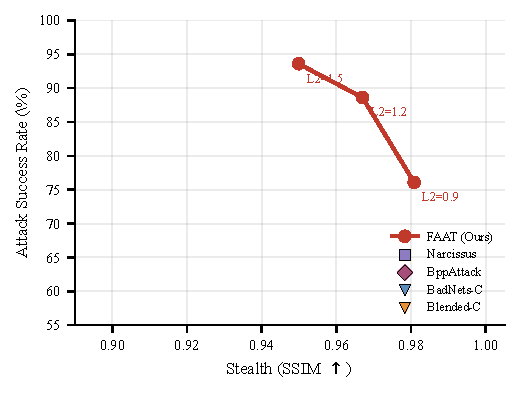
\includegraphics[width=\linewidth]{floats/figures/f4_pareto.pdf}
\caption{\textbf{Stealth--effectiveness trade-off} (CIFAR-10). FAAT (red) traces
the $\ell_2$ budget $\{0.9,1.2,1.5\}$; at its operating point it reaches
$\asr\!=\!93.6\%$ with SSIM $0.95$, dominating Narcissus and BppAttack on the
ASR--SSIM front.}
\label{fig:pareto}
\end{figure}


\paragraph{Stealth--effectiveness trade-off.}
Figure~\ref{fig:pareto} places methods on the ASR--SSIM plane. FAAT traces its
$\ell_2$ budget $\{0.9,1.2,1.5\}$; at the operating point ($\ell_2\!=\!1.5$,
SSIM $0.95$) it reaches $93.6\%$ ASR, dominating Narcissus
($\asr\!\approx\!0.88$, SSIM $0.946$) and BppAttack (SSIM $\approx\!0.97$ but
lower ASR). Lower budgets trade ASR for stealth: $\ell_2\!=\!0.9$ gives SSIM
$0.98$ at $76.1\%$ ASR, and $\ell_2\!=\!1.2$ gives $88.6\%$ at SSIM $0.967$---a
smooth, selectable frontier. The per-$\ell_2$ numbers are stable across 3 seeds
($\sigma_{\asr}\!\le\!2.5$, see supp.).
